
\newpage
%**************************************************************
\chapter{ASI SRL}
\label{cap:introduzione}
%*
\section{Presentazione Azienda}
\asi fondata a Padova nel 1989, è una società presente nel mercato dell'IT (Information Technology) da oltre 25 anni, con attività di progettazione e sviluppo di prodotti software di tipo industrializzato:
\begin{itemize}
	\item ERP (Enterprise Resource Planning, letteralmente "pianificazione delle risorse d'impresa") per aziende manifatturiere e commerciali;
	\item soluzioni per la gestione delle risorse umane;
	\item soluzioni per la gestione documenti;
	\item attività di consulenza applicativa e di processo;
	\item servizi internet a valore aggiunto;	
\end{itemize}
Queste attività hanno portato alla creazione di una propria suite di soluzioni software (denominata \textbf{Plain}), diretta principalmente ad aziende nel settore manifatturiero e commerciale, ma che fornisce numerose funzionalità anche per aziende di servizi.
\section{Struttura Aziendale}

\begin{figure}[ht]
	\centering
	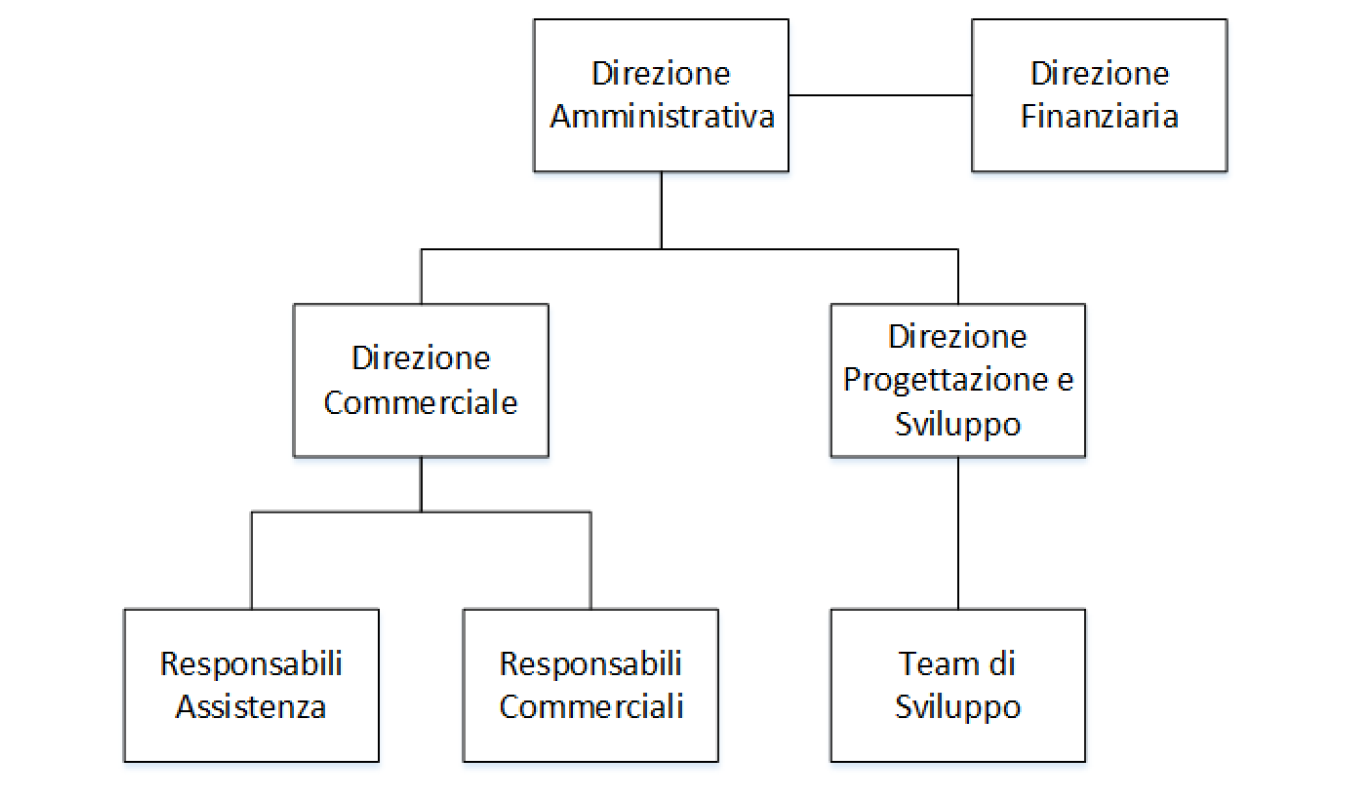
\includegraphics[scale=0.20]{immagini/azienda/struttura_aziendale}
	\caption{\textit{Struttura aziendale \asi}}
\end{figure}\FloatBarrier

Diventa partner IBM dal 1990 e partner Microsoft nel 2000, ASI ha introdotto con largo anticipo, nel 2001, l'utilizzo di servizi cloud nella gestione delle risorse umane, estendendoli in seguito anche ad altri ambiti come i servizi di logistica e di previsione della domanda.

\begin{figure}[ht]
	\centering
	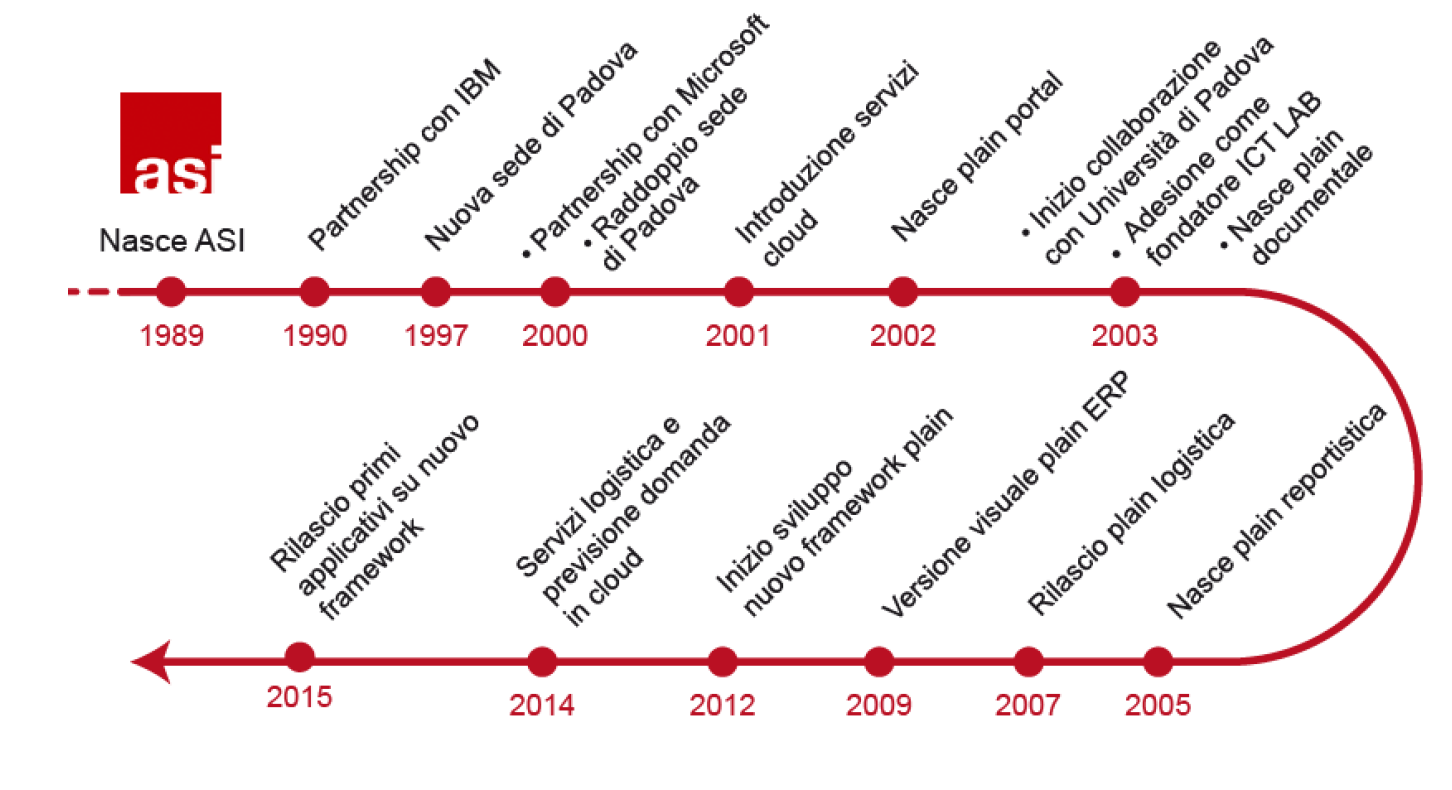
\includegraphics[scale=0.25]{immagini/azienda/timeline}
	\caption{\textit{\textit{Timeline \asi}}}
\end{figure}\FloatBarrier

ASI è associata a Confindustria ed è tra i fondatori di ICTLAB, un gruppo di aziende promosso dalla sezione dei servizi innovativi di Confindustria Padova, allo scopo di contribuire alla sviluppo di un polo produttivo Veneto nel settore delle tecnologie ICT (Information and Communication Technology, letteralmente " tecnologie dell'informazione e della comunicazione "), inoltre ASI collabora da anni con il Dipartimento di Matematica dell'università di Padova, su progetti di ricerca e sviluppo che interessano la tecnologia ed i prodotti su cui opera.
\\\\
ASI è presente principalmente in Italia settentrionale con circa 200 aziende clienti. Grazie alla flessibilità del prodotto Plain è in grado di servire sia aziende di modeste dimensioni con meno di 50 dipendenti e fatturati sotto i 5 milioni, sia aziende con oltre 500 dipendenti che superano i 50 milioni di fatturato.

\begin{figure}[ht]
	\centering
	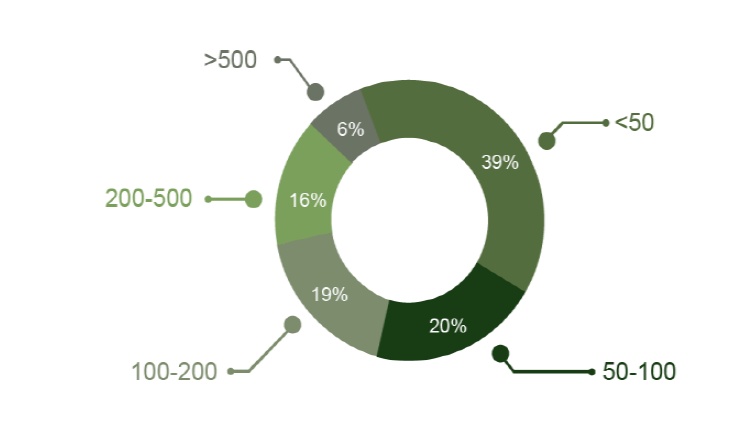
\includegraphics[scale=0.35]{immagini/azienda/dipendenti_clienti}
	\caption{\textit{Dipendenti Clienti \asi}}
\end{figure}\FloatBarrier

\begin{figure}[ht]
	\centering
	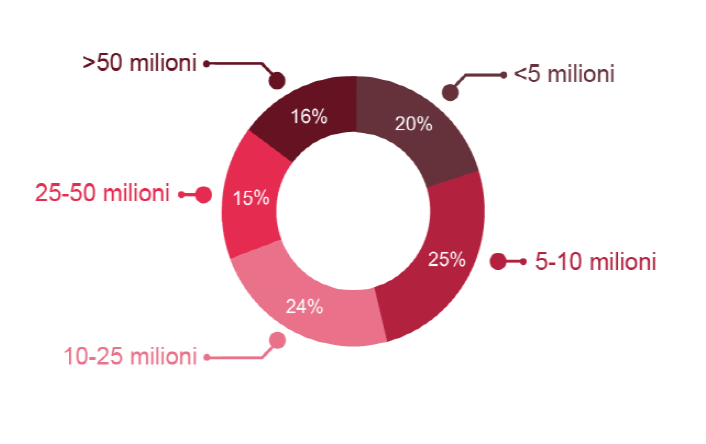
\includegraphics[scale=0.35]{immagini/azienda/fatturato_clienti}
	\caption{\textit{Fatturato Clienti \asi}}
\end{figure}\FloatBarrier

I prodotti e le soluzioni ASI sono pubblicizzati localmente tramite presenza di fiere di settore, tele-marketing mirato utilizzando aziende specializzate, passaparola di clienti soddisfatti.
\\\\
Globalmente vengono invece pubblicizzati attraverso il portale web e con campagne di annunci su Google, tramite \textit{adwords}.
\\\\
Il successo di ASI non deriva solamente dalla qualità del prodotto Plain, ma anche dall'approccio consulenziale  che utilizza con i suoi clienti e dal metodo operativo che applica ad ogni progetto intrapreso.
\section{Processi Aziendali}
\subsection{Processi interni}
Per la gestione dei propri processi aziendali, ASI ha sviluppato un sistema basato sui prodotti Plain, calibrato sulle proprie esigenze, applicando il medesimo approccio che l'azienda utilizza per i suoi clienti.
\\\\
Nel frattempo, ASI sfrutta il proprio sistema anche come ambiente di prova, sperimentando l'efficacia di nuove funzionalità in una situazione di lavoro reale.
\subsubsection{Tecnologie adottate}
Per i processi di sviluppo del proprio software, ASI applica la metodologia Scrum.\\
Si tratta di una metodologia incrementale di sviluppo agile creata da \textit{Microsoft\ped{G}}. la quale suddivide l'intero processo di creazione del software in diverse serie di attività di breve durata (Sprint), che vengono strutturate per perseguire un obiettivo generale definito in precedenza, valutando, al termine di ogni Sprint, gli incrementi ottenuti e la quantità di Sprint ancora necessarie per raggiungere l'obiettivo prestabilito.
\\\\
Tale metodologia consente di monitorare e modificare più facilmente la direzione del progetto, per meglio adattare il prodotto alle richieste del cliente.
\subsection{Processi esterni}
\subsubsection{Approccio consulenziale}
Valutata la tipologia dell'azienda cliente, ASI invia un dipendente commerciale scelto per la sua conoscenza del settore in cui opera il cliente, in modo da assicurare l'utilizzo di un linguaggio largamente condiviso, anche nelle forme gergali cui il cliente è abituato, per favorire la migliore comunicazione possibile ed una analisi più efficace delle esigenze dell'azienda contattata.
\\\\
Durante il primo approccio l'attenzione viene focalizzata non solo sui tempi di realizzazione e sui costi del progetto che si vuole intraprendere, ma anche sulle risorse dell'azienda cliente che possono essere coinvolte, in modo da condividere il più possibile la definizione degli obiettivi del progetto, ponendo il valore aggiunto di ASI sia nell'approfondita competenza tecnica e funzionale, sia nella capacità di stabilire un proficuo rapporto umano con la clientela.
\subsubsection{Startup di progetto}

\begin{figure}[ht]
	\centering
	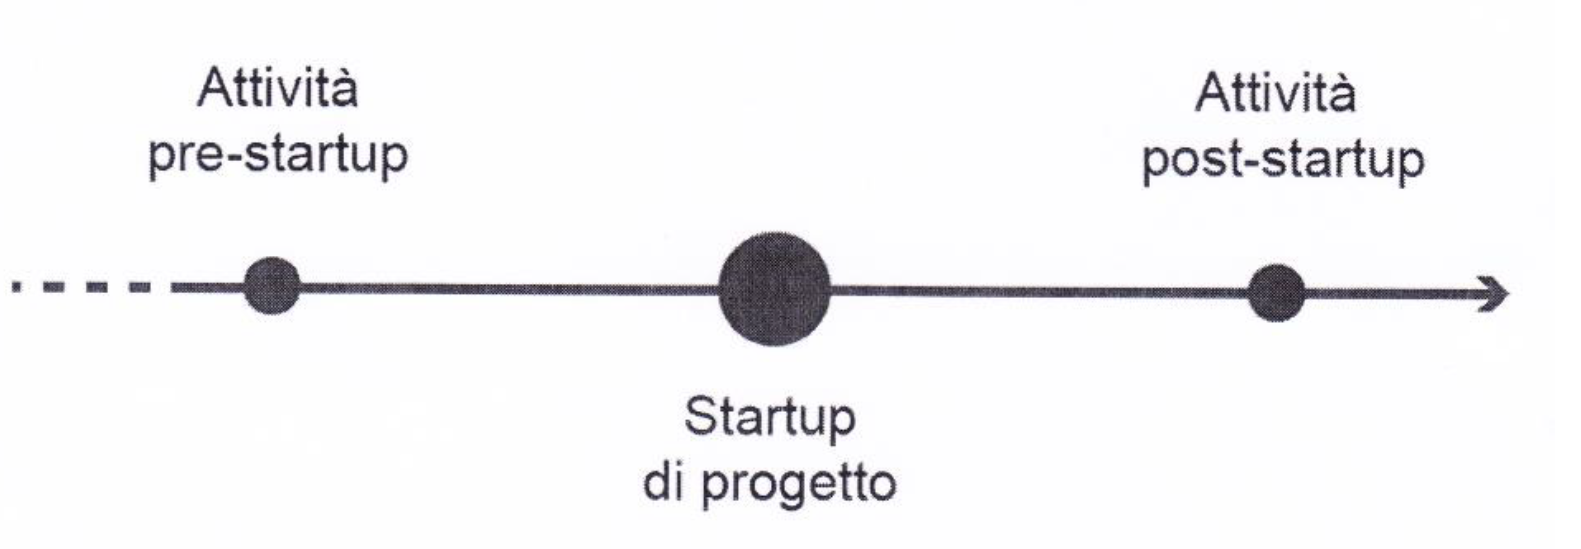
\includegraphics[scale=0.25]{immagini/azienda/startup_di_progetto}
	\caption{\textit{Startup di progetto}}
\end{figure}\FloatBarrier

Una volta confermato l'interessamento del cliente nell'applicazione di uno o più prodotti Plain, inizia lo Startup di progetto, normalmente suddiviso in tre sezioni di attività:
\begin{itemize}
	\item attività Pre-Startup;
	\item attività di Startup;
	\item attività Post-Startup;
\end{itemize}
La metodologia di progetto ASI consente di pianificare gli interventi nel modo più consono alle dimensioni e alle potenzialità dell'azienda cliente, garantendo sempre ed in ogni caso l'accesso alle migliori competenze e alle soluzioni più efficaci, senza mai rinunciare agli standard qualitativi prefissati.
\paragraph{Attività Pre-Startup}
Le attività Pre-Startup comprendono principalmente l'analisi dell'ambiente e delle necessità del cliente e la progettazione del prodotto, nel pieno rispetto dei bisogni e della struttura dell'azienda.
\\\\
Durante l'approccio consulenziale vengono definite le dimensioni e le possibilità economiche e strutturali dell'azienda, dando una prima definizione della complessità del progetto da intraprendere, adattando di conseguenza lo sforzo delle risorse di ASI.
\\\\
Viene quindi designato un adeguato numero di coordinatori di progetto, a seconda della complessità rilevata; al minimo due: uno di riferimento commerciale per l'azienda cliente, solitamente il dipendente che ha effettuato l'approccio consulenziale, ed uno di riferimento tecnico.
\\\\
In caso di progetto ad alta complessità, possono essere incaricati diversi coordinatori, in modo che ciascuno copra una specifica area tecnica per poter meglio gestire il lavoro; uno di loro assume il ruolo di direttore di progetto per organizzare le varie attività dei coordinatori;
\\\\
Una volta individuate queste figure, grazie alla loro esperienza tecnica viene analizzata in dettaglio la direzione dell'azienda cliente, per ottenere una lista più dettagliata degli obiettivi e delle priorità di quest'ultima, e si prendono in esame eventuali sistemi preesistenti, per favorire una più semplice rivelazione dei fabbisogni informativi ed una migliore definizione della struttura tecnologica da adottare; vengono inoltre individuate le funzioni aziendali coinvolte e le eventuali deleghe necessarie per avviare il progetto.

\paragraph{Attività Startup}
Le attività di Startup comprendono le attività di pianificazione e gestione del lavoro oltre che l'effettiva installazione degli applicativi e la formazione del personale.
\\\\
Sfruttando le analisi effettuate nelle attività di Pre-Startup viene redatto un piano di lavoro che definisce in dettaglio:
\begin{itemize}
	\item le attività da svolgere, aspetti organizzativi del progetto e le relative tempistiche;
	\item i ruoli e le responsabilità delle risorse coinvolte nel progetto, siano esse di ASI o dell'azienda cliente;
	\item l'eventuale conversione di archivi informativi preesistenti in formati fruibili dai prodotti Plain;
	\item la stesura della documentazione di planning del progetto;
	\item la presentazione del progetto ai partecipanti ed eventuali interessati;
\end{itemize}
Si procede inoltre ad effettuare una mappatura dei processi coinvolti per poter meglio gestire il progredire delle attività in corso, arrivando infine all'installazione dei programmi applicativi, durante la quale viene inizialmente creato un ambiente di prova per testare le piene funzionalità dei prodotti da installare e, solo successivamente, si svolge la parametrizzazione ed installazione del sistema prodotto.
\\\\
Infine avviene la stesura della documentazione di configurazione del sistema e della documentazione sulle scelte di intervento ed i relativi vantaggi attesi.
\\\\
Al termine dell'installazione del sistema vengono avviate attività di sviluppo di eventuali funzionalità addizionali personalizzate per l'azienda cliente.
\\\\
Le ultime attività di Startup comprendono la formazione del personale ed il collaudo in loco del sistema.
\\\\
Sono inoltre previste sessioni specifiche per ciascun utente delle aree coinvolte, in modo che il personale chiave dell'azienda cliente sia perfettamente in grado di utilizzare il prodotto in tutte le sue funzionalità; viene eventualmente fornita a corredo una documentazione specifica per esigenze di maggiore chiarezza sulle procedure operative del sistema e sulle regole aziendali da mantenere.
\\\\
Vengono infine effettuate operazioni di verifica di tutte le funzionalità inserite nel sistema e, solamente dopo aver ottenuto conferma della piena operatività, il sistema viene effettivamente avviato all'interno dell'azienda cliente.

\paragraph{Attività Post-Startup}
Le attività di Post-Startup comprendono le attività di ulteriore personalizzazione e perfezionamento del sistema informatico installato, assicurando che le funzionalità del prodotto corrispondano esattamente alle esigenze del cliente.
\\\\
Viene inoltre offerto un piano di supporto calibrato sulle possibilità dell'azienda, iniziando da soluzioni più standardizzate arrivando ad una serie di strumenti elaborati ad hoc, mantenendo in ogni caso un affiancamento tecnico agli utenti aziendali per garantire la massima tranquillità operativa di questi ultimi.
\\\\
Si concorda infine con il cliente un piano di mantenimento e di verifica del sistema, la cui durata può variare da uno a diciotto mesi, secondo la complessità definita precedentemente.

\section{Plain}
Plain è una suite di soluzioni software sviluppata da \asi per supportare principalmente la gestione delle aziende che hanno specifiche competenze in ambiti produttivi e commerciali; tutti i prodotti forniti condividono una serie di caratteristiche e funzionalità che li accomunano e che ne qualificano la metodologia di sviluppo.

\subsection{Caratteristiche}
Le soluzioni Plain sono caratterizzate da un'architettura scalabile ed aperta all'utilizzo in rete, in grado di gestire efficacemente un qualsiasi volume di utenti o dati, anche su cloud, per permettere la fruibilità ad aziende di qualsiasi dimensione; forniscono inoltre un'ampia configurabilità per permettere:
\begin{itemize}
	\item una profonda adattabilità al contesto organizzativo in cui vengono inserite, in modo da adattarsi sia alla tipologia dell'azienda, sia agli eventuali sistemi informatici già utilizzati, modificando il meno possibile le abitudini dei clienti;
	\item un'alta navigabilità, puntando ad ottenere tutte le informazioni disponibili, collegate ad un soggetto (un cliente, un fornitore, un articolo o altro), il più efficacemente possibile;
	\item una gestione puntuale della sicurezza e riservatezza nell'accesso ai dati, sia all'interno, che all'esterno dell'azienda;
\end{itemize}
Le soluzioni Plain inoltre contengono una serie di funzionalità condivise:
\begin{itemize}
	\item la personalizzazione delle interfacce utente, come i cruscotti aziendali, le KPI (Key Performance Indicatrors o indicatori chiave di prestazioni), le relazioni tra documenti e la navigabilità, che consente di aver un sistema a supporto dell'utente e non il contrario;
	\item gestione documentale, reportistica (analisi e statistiche) e KPI integrate nella soluzione gestionale e disponibili in ogni momento per restituire informazioni contestualizzate;
	\item modulo BPM (Business Process Management) integrato per la modellazione dei flussi di lavoro;
	\item connettori con soluzioni specialistiche dipartimentali, come la tesoreria, CRM (Customer Relationship Management o gestione delle relazioni con i clienti), e-commerce etc.;
	\item base di dati accessibile da qualsiasi piattaforma con strumenti di analisi o Business Intelligence;
\end{itemize}
\subsubsection{Soluzioni Plain principali}
\begin{itemize}
	\item \textbf{Plain ERP industria}, si tratta di una piattaforma creata per fornire supporto a tutte le attività gestionali di un'azienda di produzione industriale, raccogliendo i moduli applicativi in 8 aree funzionali (amministrazione, finanziaria, di controllo, vendite, approvvigionamenti, magazzino, produzione ed integrazione), con specializzazione negli ambiti della produzione metalmeccanica, sia in serie che su commessa, e sullo stampaggio ed estrusione di materie plastiche.
	
	\begin{figure}[ht]
		\centering
		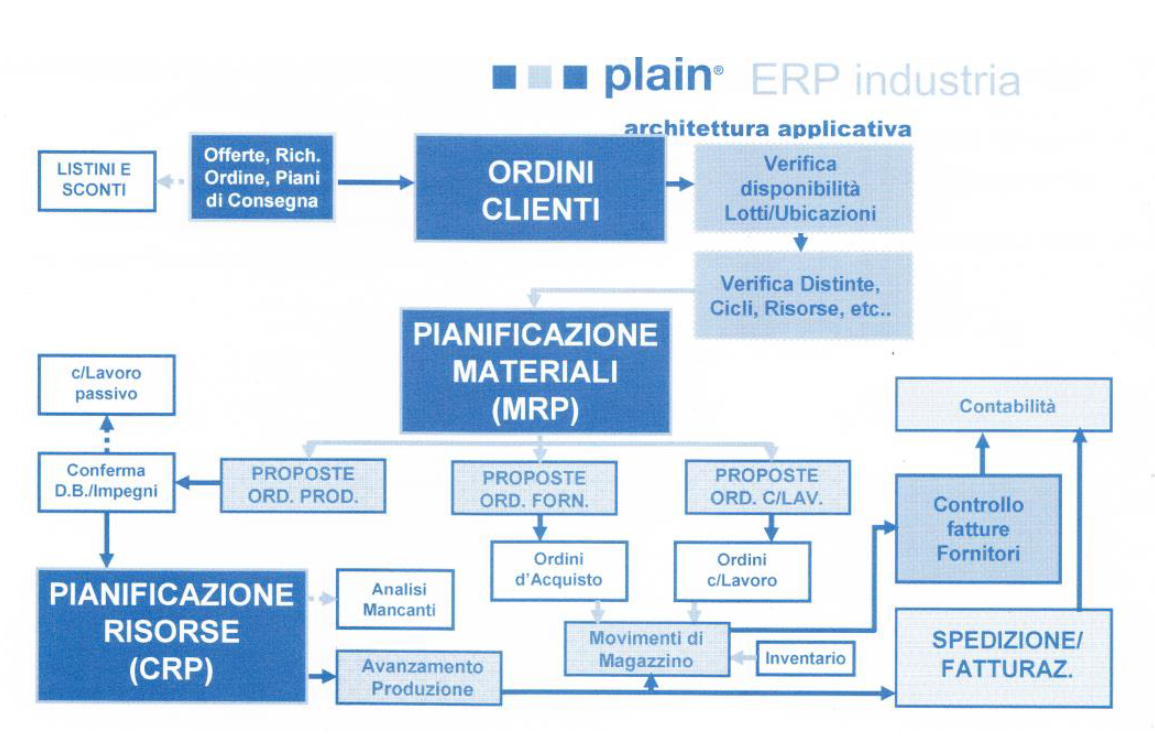
\includegraphics[scale=0.40]{immagini/azienda/plain_erp_industria}
		\caption{\textit{Plain ERP Industria}}
	\end{figure}\FloatBarrier
	
	\item \textbf{Plain ERP Commercio}, soluzione specificatamente destinata alle attività gestionali di un'azienda commerciale, i cui moduli applicativi sono raccolti in 9 aree funzionali (amministrazione, finanziaria, di controllo, vendite, approvvigionamenti, magazzino, assistenza tecnica, lavorazioni ed integrazione), con specializzazione nei mercati della carta e cancelleria (grossisti, fornituristi e cash), giocattoli ed articoli da regalo, ricambi (sia automotive che industriali), nonché ferramenta ed utensileria.
	
	\begin{figure}[ht]
		\centering
		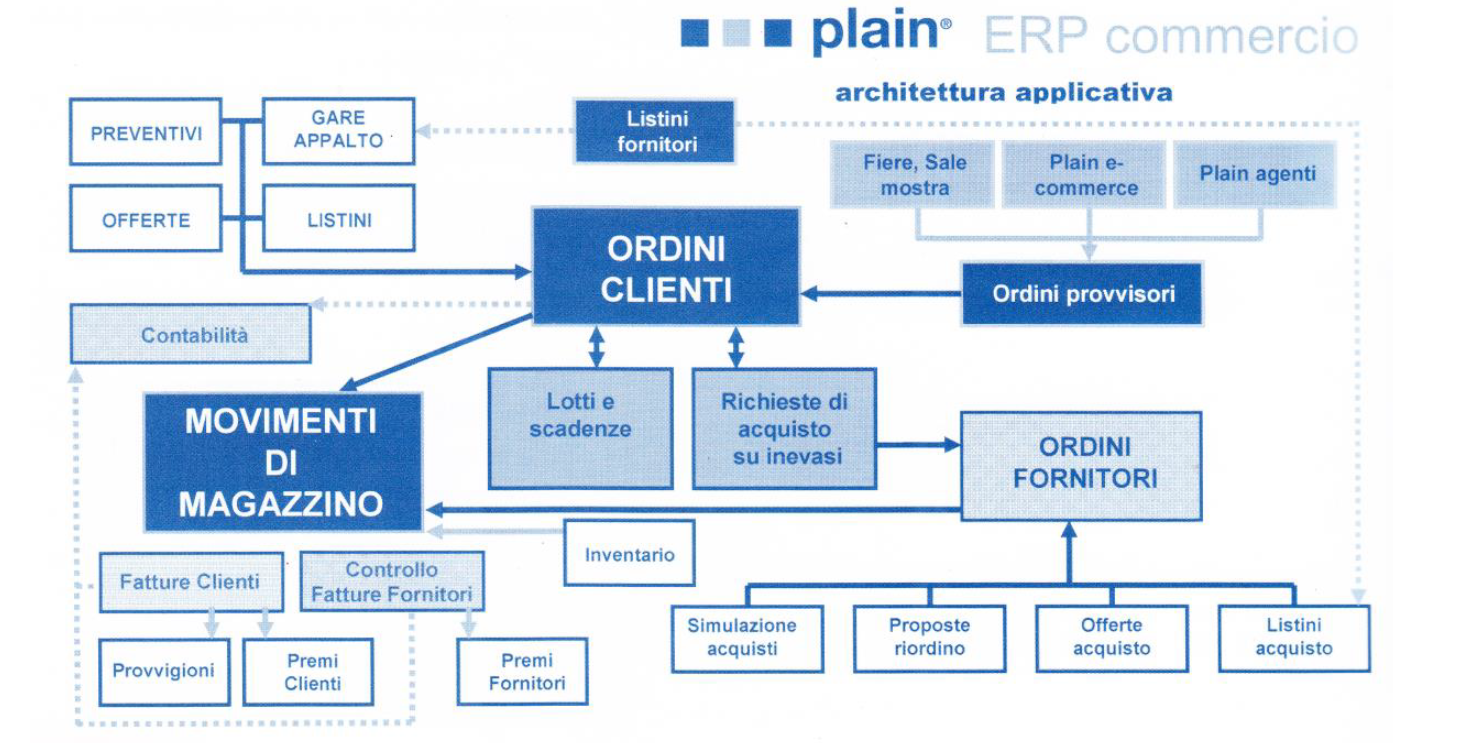
\includegraphics[scale=0.35]{immagini/azienda/plain_erp_commercio}
		\caption{\textit{Plain ERP Commercio}}
	\end{figure}\FloatBarrier
	
\end{itemize}
\subsubsection{Altre soluzioni Plain}
Plain fornisce ulteriori soluzioni applicabili in qualsiasi ambito aziendale oppure destinate a specifiche tipologie di azienda; queste soluzioni possono essere di supporto anche ai due principali ERP Plain, applicabili singolarmente o interfacciate con ERP già esistenti:
\begin{itemize}
	\item Plain Logistica, studiata principalmente per grossisti di carta e cancellerie o fornituristi di ufficio, fornisce un sistema per la migliore gestione dei magazzini e dei processo di movimento della merce;
	\item Plain Previsione Domanda, studiata principalmente per grossisti di carta e cancellerie o fornituristi di ufficio, fornisce un sistema per tracciare ed analizzare le vendite ed acquisti, per rendere più efficace ed efficiente gestire le richieste dei clienti;
	\item Plain Documentale, applicabile in qualsiasi ambito aziendale, fornisce un sistema efficiente per archiviare, gestire, accedere e condividere i documenti aziendali;
	\item Plain HR (human resource), applicabile in qualsiasi ambito aziendale, fornisce un sistema per gestire tutti gli aspetti riguardanti le risorse umane in azienda;
	\item Plain Extended data publisher, applicabile in qualsiasi ambito aziendale, fornisce un sistema per gestire ed ottenere facilmente ed efficacemente le informazioni contenute nei sistemi informativi aziendali in qualsiasi momento;
	\item Plain Presenze, applicabile in qualsiasi ambito aziendale, fornisce un sistema per la rilevazione delle presenze interfacciabile con qualsiasi sistema di rilevamento delle timbrature, automatizzando i controlli periodici sulle risorse;
\end{itemize}
\subsection{Propensione all'innovazione}
ASI punta principalmente a mantenere efficace e competitiva la propria suite di prodotti Plain, sfruttando la sua adattabilità per adeguarsi alla tecnologia utilizzata nelle aziende clienti.
\\\\
L'azienda monitora costantemente le nuove tecnologie rilasciate sul mercato, cercando di individuare quelle che possano essere assimilate in tutto o in parte nella propria suite di prodotti, o che possano costituire la base per lo sviluppo di un nuovo prodotto Plain.
\\\\
Grazie al suo crescente successo, ASI è stata in grado di investire una sempre maggiore percentuale del suo fatturato nella ricerca e sviluppo dei prodotti Plain, raggiungendo circa il 22\% nel 2015; mantenendo così la suite Plain in costante evoluzione, grazie ad almeno tre aggiornamenti all'anno.
\\\\
Per valutare l'efficacia e l'eventuale utilizzo di nuove tecnologie, ASI svolge innanzitutto una prima analisi per individuare in dettaglio le funzionalità e caratteristiche che possono portare migliorie o aggiunte all'interno dei prodotti Plain, cercando di definire i costi e la quantità di lavoro necessaria per la loro implementazione.
\\
Se l'analisi effettuata porta risultati soddisfacenti vengono allestiti progetti per sviluppare implementazioni di prova, i quali possono essere portati a termine interamente da membri del team di sviluppo, ma che spesso vengono proposti come esperienze di stage tramite l'Università di Padova.

